\subsection{Differences between UAM, AA and UAV}

\Gls{UAM} differs from traditional aircrafts with its use of rotors, and the ability to take off and land vertically from almost anywhere with a suitable platform, such as vertiports, and helipads, whereas traditional aircrafts are mostly equipped with fixed wings and require runways to operate \cite{Schuchardt_2023}.
Its range of opperation also differs, with \gls{UAM} operate in urban areas (intra- and inter-city) while traditional aircrafts are able to operate for long distance travel, but only to locations with runway availability.
Fig.~\ref{fig:venn-diagram} shows the comparison between \gls{UAM}, \gls{UAV} and conventional aircrafts.
Fig.~\ref{fig:airspace-mobility} shows the distance which the aircrafts travel to and from, as well as the airspace it occupies.

\begin{figure}[h]
    \centering
    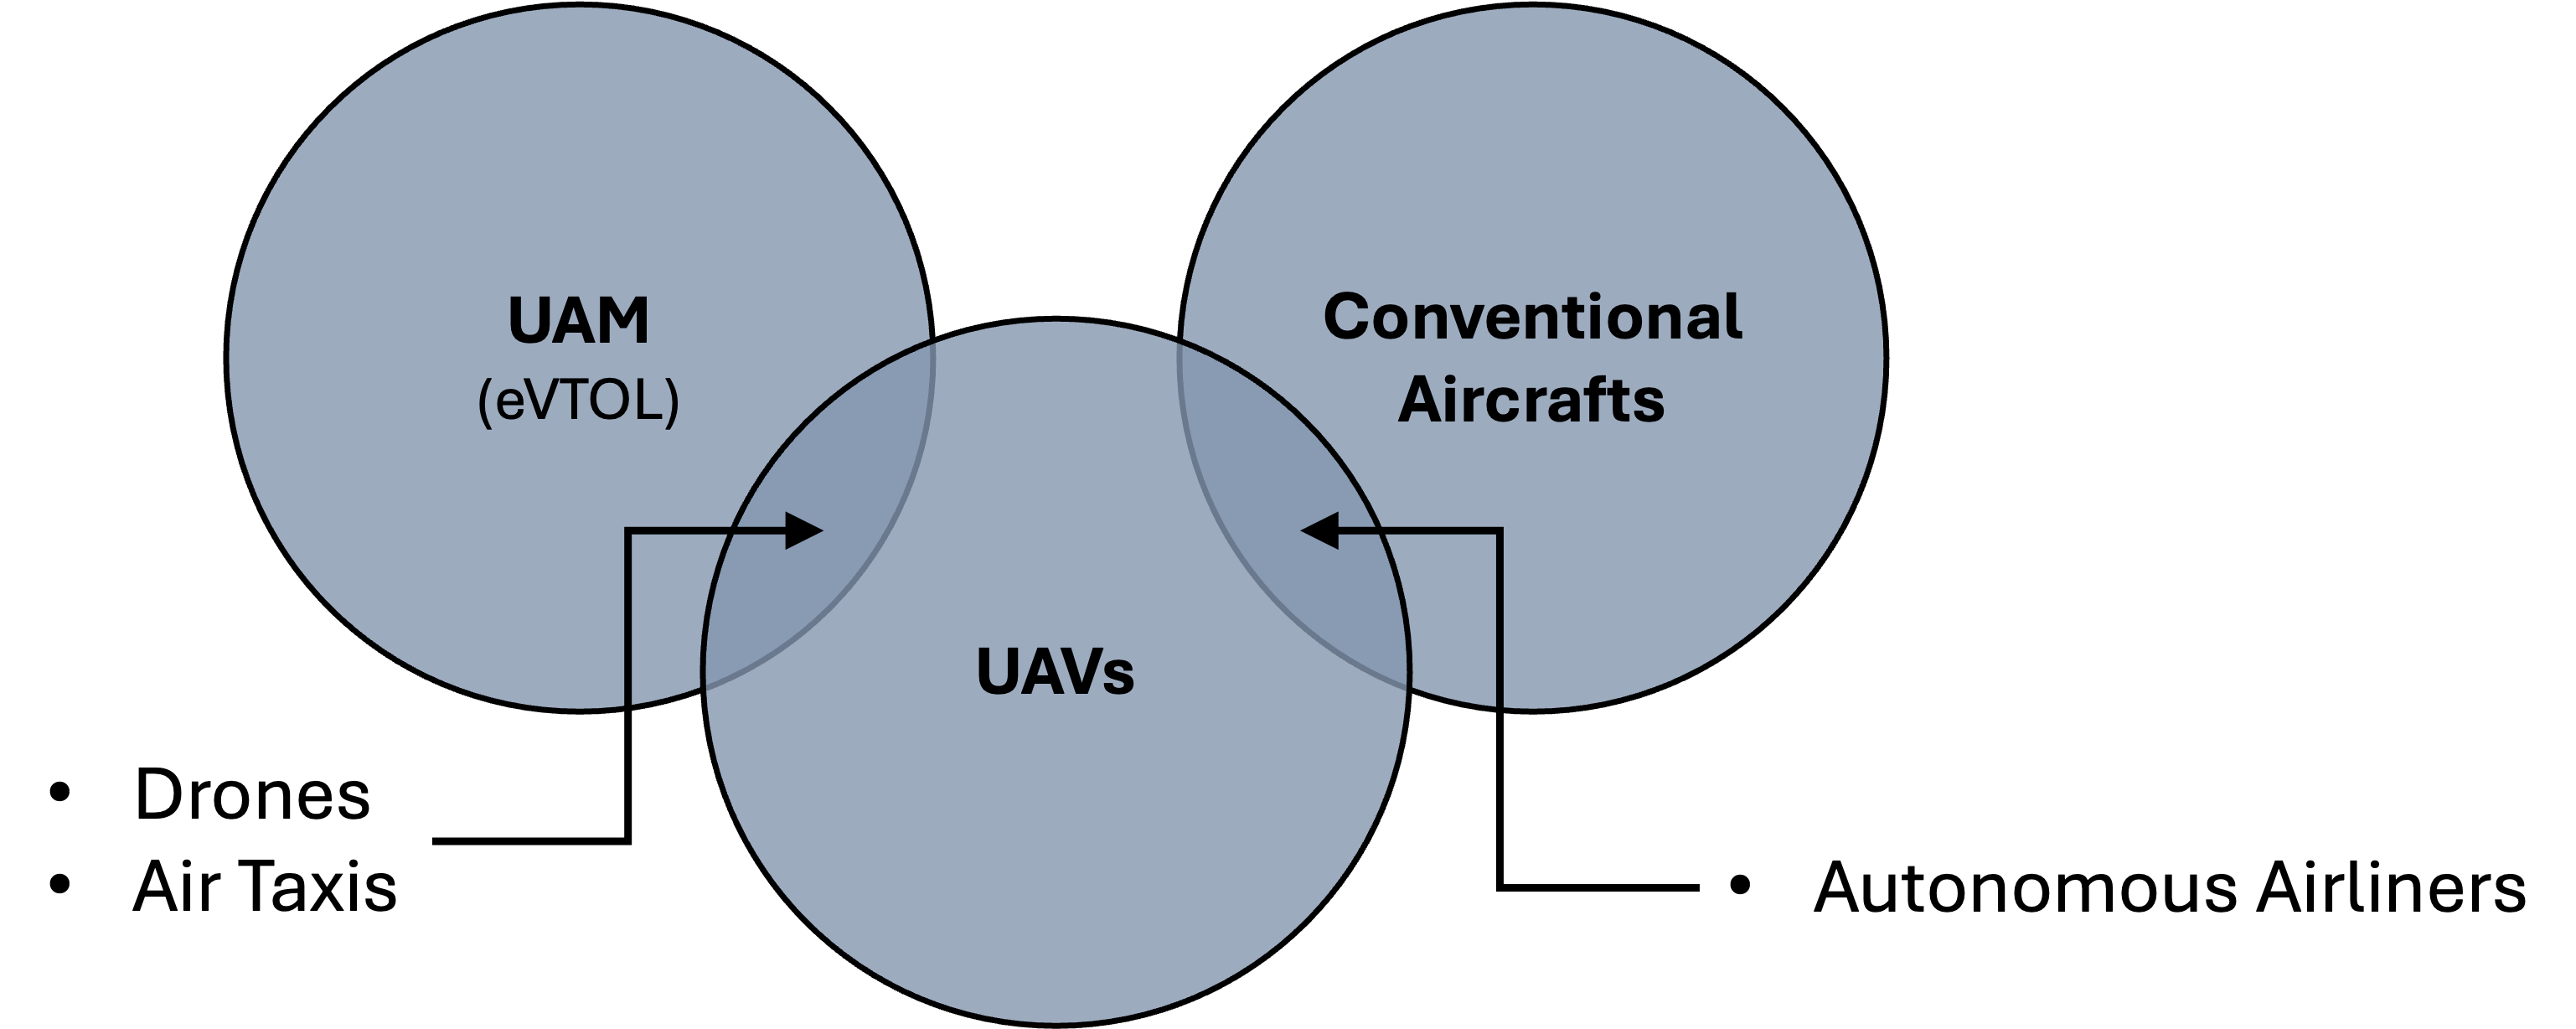
\includegraphics[width=.6\textwidth]{venn-diagram.png}
    \caption{Venn diagram of \gls{UAM}, \gls{UAV} and conventional aircrafts.}
    \label{fig:venn-diagram}
\end{figure}

\begin{figure}[h]
    \centering
    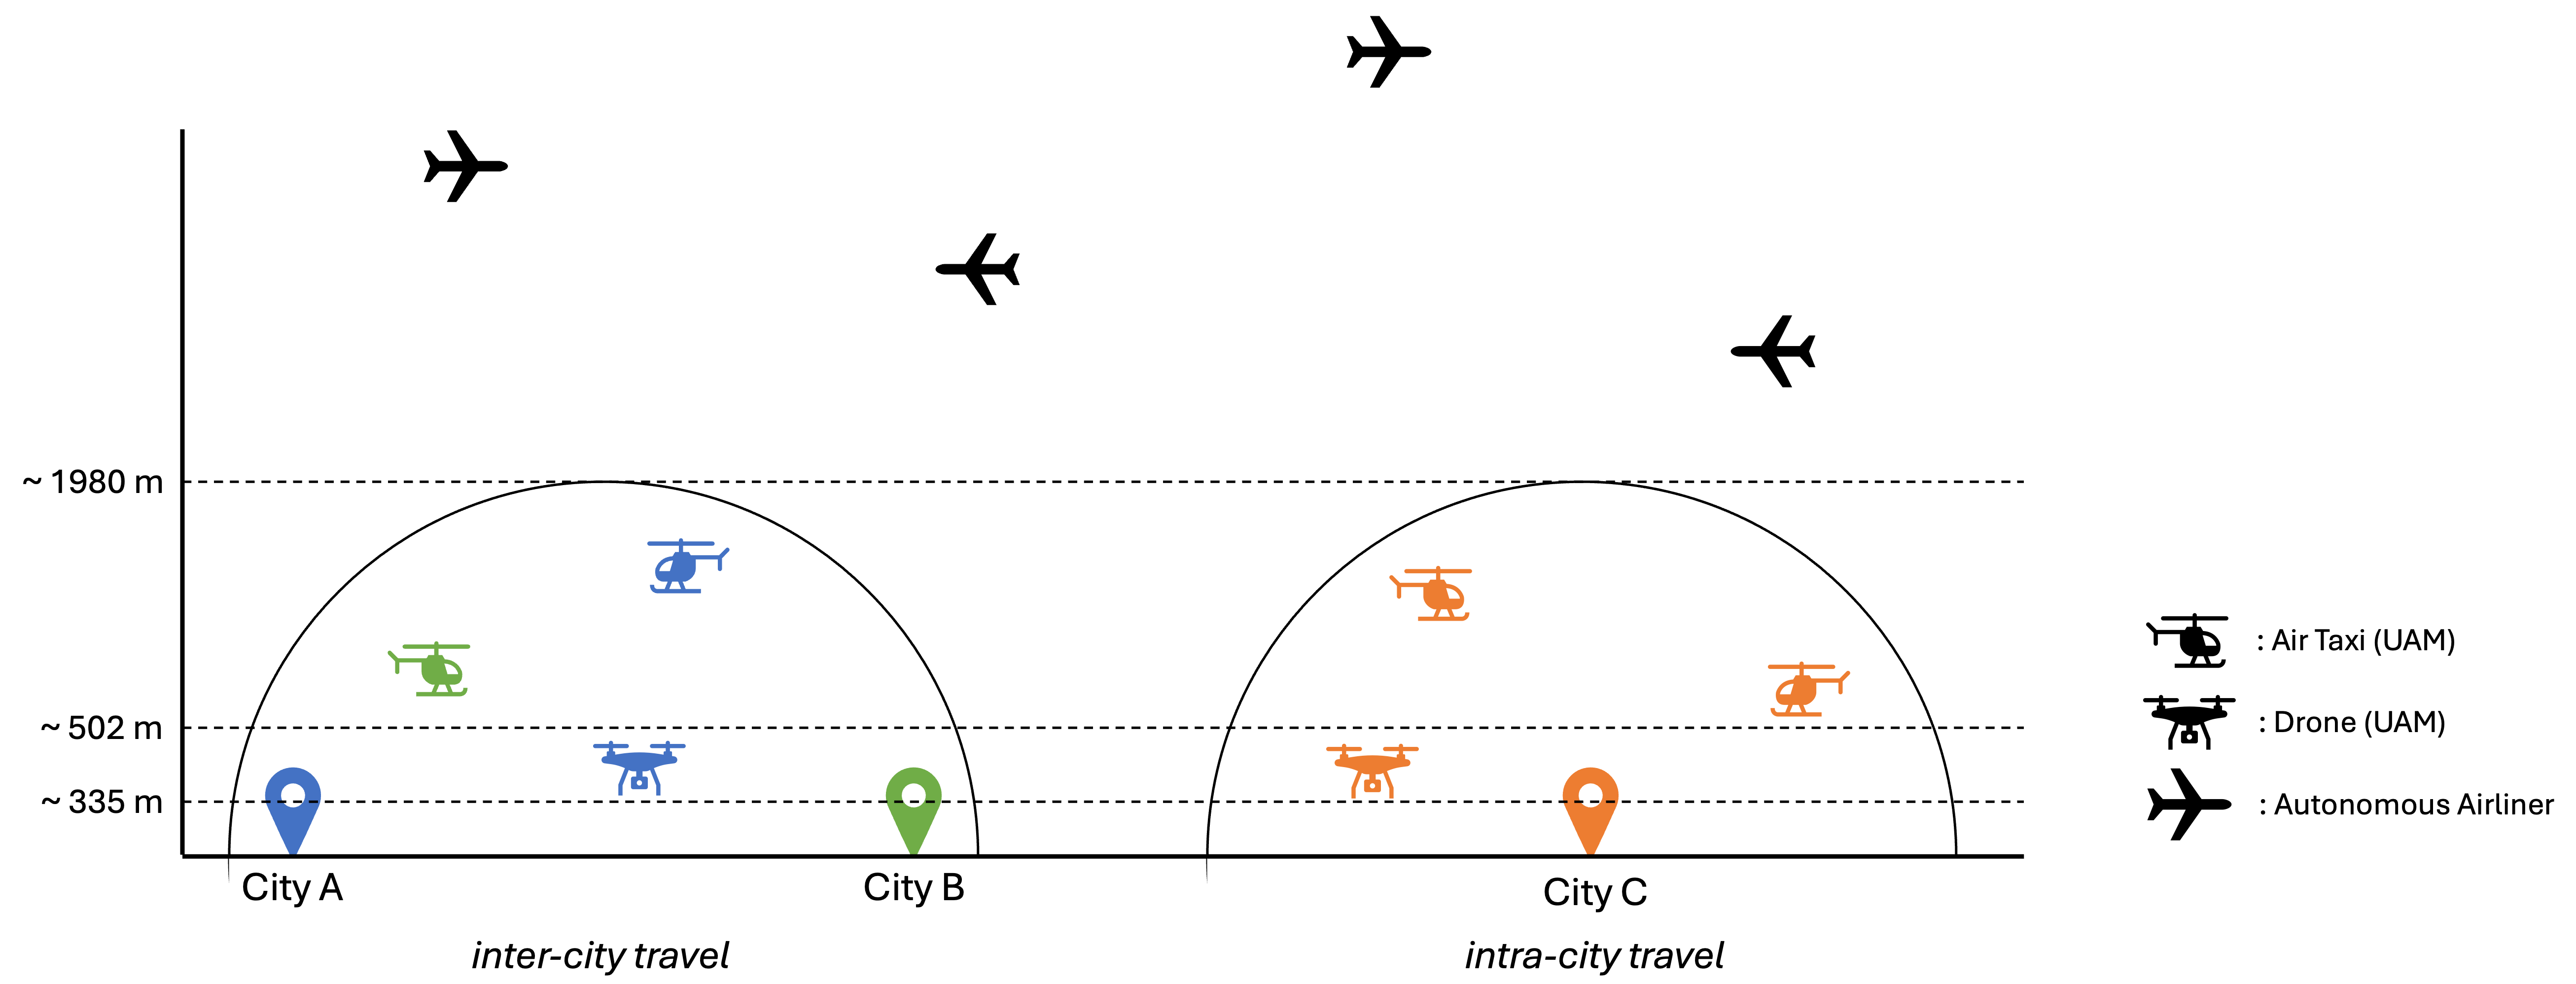
\includegraphics[width=\textwidth]{airspace-mobility.png}
    \caption{Mobility of \gls{UAM} and autonomous airliners.}
    \label{fig:airspace-mobility}
\end{figure}
